%%% Folie
\begin{frame}{Ausgangslage}
    Nach dem Einstieg in Python und IoT über Kapitel 3 und 4 sollen nun in diesem Kapitel fortgeschrittene Konzepte aufgezeigt werden, mit deren Hilfe die jeweilige Code-Basis geordnet wachsen kann und Abläufe mit Hilfe von Konzepten aus der nebenläufigen Programmierung gezielt optimiert werden können.

    \end{frame}

%%% Folie
\begin{frame}{Lernziele}
    \begin{itemize}
        \item Komplexe Anwendungsfälle objektorientiert modellieren können
        \item Python-Anwendungen mit Klassen und Modulen modularisieren können
        \item Die Nachteile einer zu engen Kopplung von Klassen verstehen können
        \item Entwurfsmuster Observer und Message Broker anwenden können
        \item Nebenläufige Programmierung mit Threads in Python
        \item Nebenläufige Programmierung mit Coroutines in Python
    \end{itemize}
\end{frame}


%-------------------------------------------------------------------------------
\section{Design Patterns}
%-------------------------------------------------------------------------------

%%% Folie
\begin{frame}{Design Patterns in Python}
    \begin{itemize}
        \setlength{\itemindent}{2.25in}
        \item [\textbf{Motivation: Design Patterns in Python}]
    \end{itemize}

    \begin{itemize}
        \item Sehr langen, schwer wartbaren Source Code vermeiden, denn Python ist flexibel und kann insbesondere für Skripte verwendet werden  $\Rightarrow$  Eine saubere Struktur hilft
        \item Refactoring vereinfachen  $\Rightarrow$  Besser wenige oder eine Klasse anpassen, als alles (am besten ohne Tests \smiley{} )
        \item Teamarbeit vereinfachen  $\Rightarrow$  Wenn  nicht ständig mit anderen an derselben Datei editiert werden muss, kommt es zu weniger Merges im git repository
   \end{itemize}

  \end{frame}


%%% Folie
\begin{frame}{Enge Kopplung}
    	  \begin{figure}[!htb]
        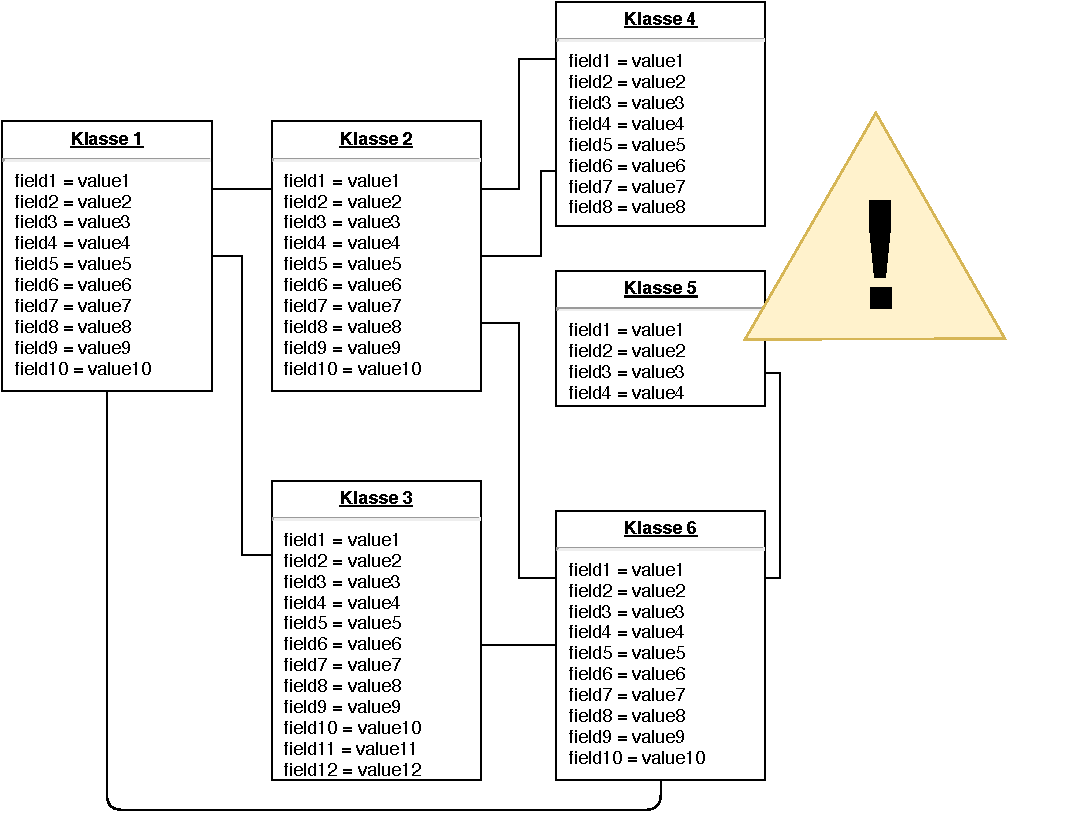
\includegraphics[scale=0.5]{img/tightcoupling}
    \end{figure}
\end{frame}


%%% Folie
\begin{frame}{Dependency Injection}
 \begin{itemize}
        \setlength{\itemindent}{1.3in}
        \item [\textbf{Dependency Injection}]
    \end{itemize}

    \begin{itemize}
        \item Bindung an Abhängigkeiten wird reduziert durch Schnittstellen (Funktionen und Objekte als Parameter)
        \item Boilerplate Code an falscher Stelle wird vermieden
        \item In viele Programmiersprachen existieren Frameworks (z.B. Spring Autowiring, Dagger oder Guice für Java)
        \item Injection Frameworks in Python aufgrund der Beschaffenheit der Sprache unüblich
   \end{itemize}

\end{frame}


%%% Folie
\begin{frame}{Inversion Of Control}
\begin{itemize}
        \setlength{\itemindent}{1.25in}
        \item [\textbf{Inversion Of Control}]
    \end{itemize}

    \begin{itemize}
        \item Nichtprozedurale Programmierstile werden gefördert (z.B. eventbasiert)
        \item Programme sind modularer
        \item Auch Frameworks sind bspw. eine Form von IOC
   \end{itemize}

\end{frame}


%%% Folie
\begin{frame}{Besonderheiten in Python: Ducktyping}
  \begin{itemize}
        \setlength{\itemindent}{1.2in}
        \item [\textbf{Recap: Ducktyping}]
    \end{itemize}

    \begin{itemize}
        \item In Python reichen gleiche Funktionsnamen als Schnittstelle aus zwischen Parameterempfänger und Funktion/Objekt im Argument
        \item Typen spielen hier keine Rolle
    \end{itemize}

  \end{frame}


  %%% Folie
\begin{frame}{Besonderheiten in Python: Monkey Patching }
  \begin{itemize}
        \setlength{\itemindent}{1.1in}
        \item [\textbf{Monkey Patching}]
    \end{itemize}

    \begin{itemize}
        \item In Python kann man wie in JavaScript zur Laufzeit Attribute oder Methoden an Objekte \quotes{patchen}
        \item Die alte Funktion/der alte Wert wird somit ersetzt
        \item Effektiv besteht somit ein \textbf{Hook} für beliebige Funktionen
        \item Es ist Vorsicht geboten mit derartigen Möglichkeiten
    \end{itemize}

  \end{frame}


   %%% Folie
\begin{frame}{Besonderheiten in Python: Mixins}
   \begin{figure}[!htb]
        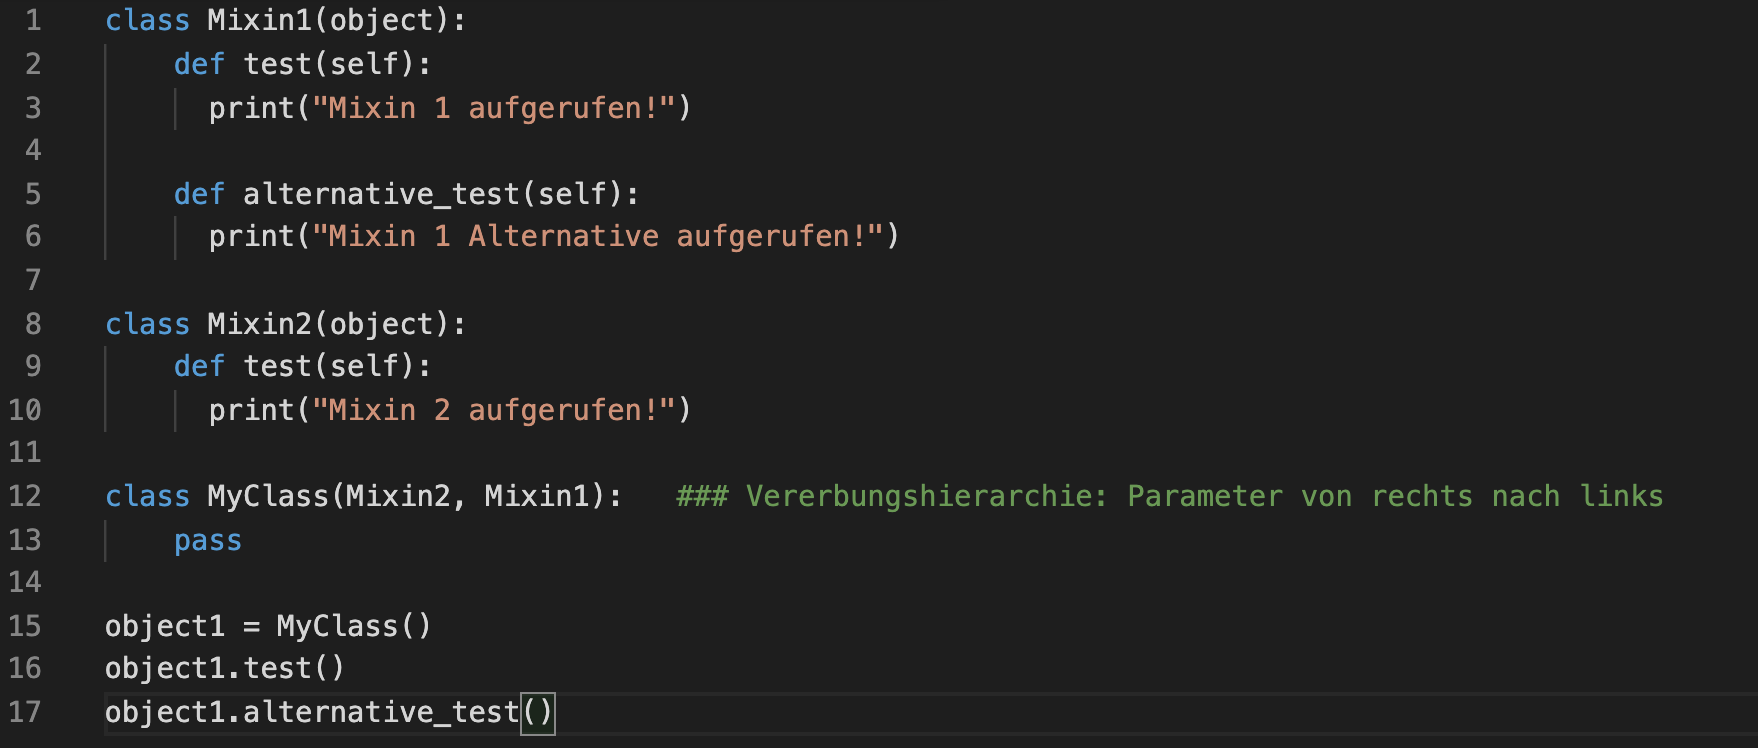
\includegraphics[scale=0.37]{img/mixins}  %https://www.ianlewis.org/en/mixins-and-python
    \end{figure}

  \end{frame}


%%% Folie
\begin{frame}{Anwendungsfall: Testing mit MagicMock}
   \begin{figure}[!htb]
        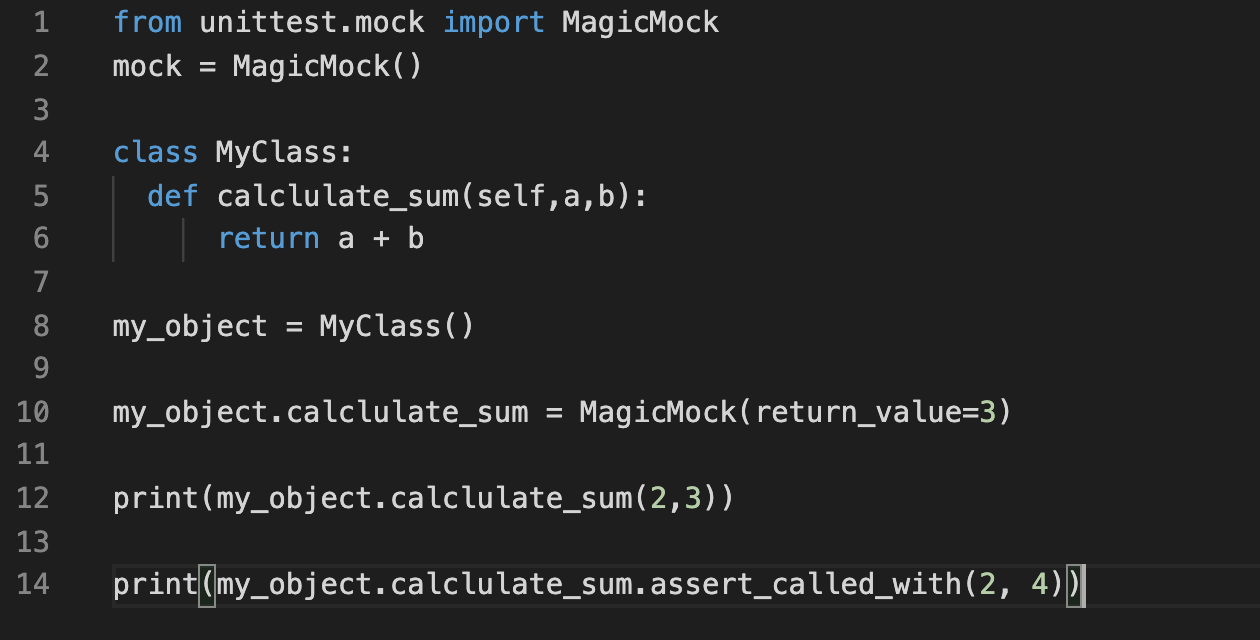
\includegraphics[scale=0.47]{img/magicmock}
    \end{figure}

\end{frame}

%%% Folie
\begin{frame}{Observer Pattern 1}
       \begin{figure}[!htb]
        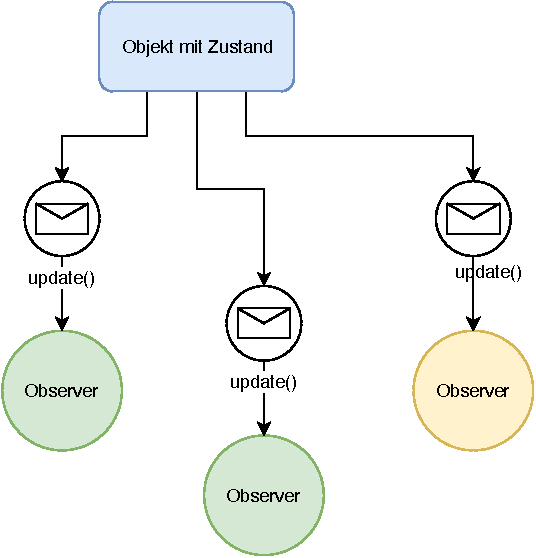
\includegraphics[scale=0.67]{img/observer}
    \end{figure}

\end{frame}

%%% Folie
\begin{frame}{Observer Pattern 2}
        \begin{itemize}
        \setlength{\itemindent}{1.1in}
        \item [\textbf{Observer Pattern}]
    \end{itemize}

    \begin{itemize}
        \item Losere Kopplung wird erreicht durch einheitliche Interface Methode(n)
        \item Auf Objektebene kennt aber jeder Observer das Observable   $\Rightarrow$ gewisse Kopplung bleibt zur Laufzeit erhalten - in Python ist aber der Code dank Ducktyping bereits sehr \quotes{dependency-arm}
        \item Alternative Bezeichnungen: Registry, Listener
    \end{itemize}
\end{frame}

%%% Folie
\begin{frame}{Publish-Subscribe 1} % https://hackernoon.com/observer-vs-pub-sub-pattern-50d3b27f838c
      \begin{itemize}
        \setlength{\itemindent}{1.5in}
        \item [\textbf{Publish/Subscribe Pattern}]
    \end{itemize}

    \begin{itemize}
        \item Pub/Sub ist dem Observer Pattern ähnlich, es ist aber \textbf{nicht} damit identisch
        \item Zusätzliche Abstraktion ist eine 3. Komponente zwischen Observable und Observer: der  \textbf{Message Broker}
        \item Nachrichten werden über den kommunizierenden bekannte Topics oder definierte Events ausgetauscht
    \end{itemize}

\end{frame}


%%% Folie
\begin{frame}{Publish-Subscribe 2}
      \begin{figure}[!htb]
        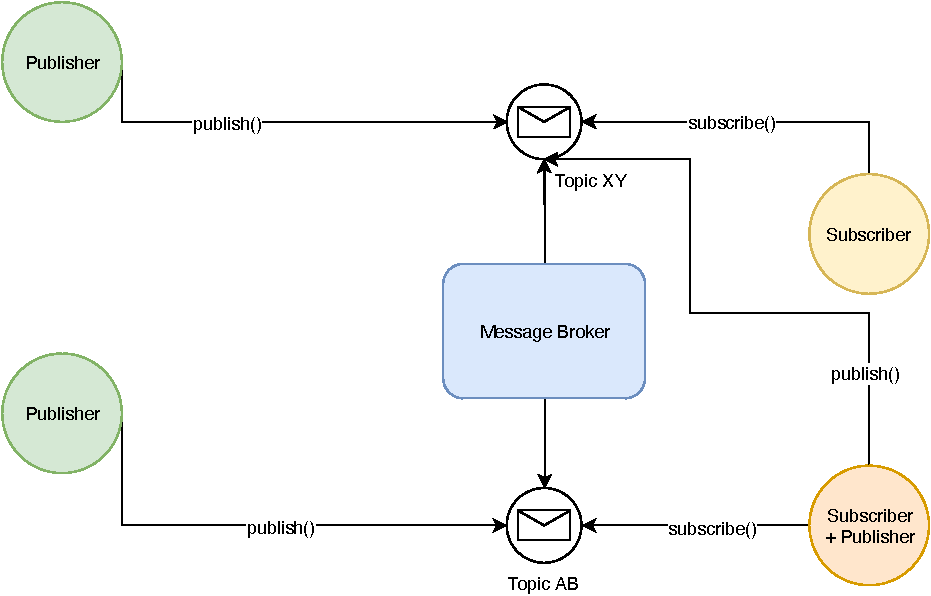
\includegraphics[scale=0.67]{img/pubsub}
    \end{figure}

\end{frame}


%%% Folie
\begin{frame}{Strukturierung der Anwendung mit Patterns}
      \begin{itemize}
        \setlength{\itemindent}{1.5in}
        \item [\textbf{Einsatz der Patterns}]
    \end{itemize}

    \begin{itemize}
        \item Dependency Injection (Übergabe von Funktionen als Parameter): Möglichst in der Datenhaltungsschicht, um Teile austauschen zu können, z.B. File Format, DB
        \item Mixins: Feature minimalinvasiv an bestehenden Code hinzufügen, Kompatibilität mit externen Modulen herstellen
        \item Monkey Patching:  bei Tests indirekt durch Mocks
        \item Observer:  wenn ein Zustand über viele Instanzen aktualisiert werden soll ...
        \item Pub/Sub:  Es werden komplexere Nachrichten benötigt und Nebenläufigkeit  wird benötigt
    \end{itemize}

\end{frame}


%-------------------------------------------------------------------------------
\section{Nebenläufigkeit in Python}
%-------------------------------------------------------------------------------

%%% Folie
\begin{frame}{Nebenläufigkeit vs. Parallelität - Intro}
        \begin{itemize}
        \setlength{\itemindent}{2.0in}
        \item [\textbf{Definition: Nebenläufig vs. Parallel}]
    \end{itemize}

    \begin{itemize}
        \item Als \textbf{nebenläufig} definieren wir Aufgaben, die auf einem Computer um Ressourcen konkurrieren und nicht notwendigerweise gleichzeitig ausgeführt werden (können). Der Fokus liegt auf dem Ausführen und Organisieren mehrerer eventuell unabhängiger Aufgaben
        \item Als \textbf{parallel} definieren wir nebenläufige Aufgaben, die gleichzeitig ausgeführt werden (können). Der Fokus liegt aber auf Leistung.
     \end{itemize}
\end{frame}

\begin{frame}{Nebenläufigkeit vs. Parallelität - Beispiele}
        \begin{itemize}
        \setlength{\itemindent}{2.2in}
        \item [\textbf{Beispiele: Nebenläufig oder Parallel?}]
    \end{itemize}

    \begin{itemize}
        \item Abfrage der Werte verschiedener angeschlossener Sensoren $\Rightarrow$ nebenläufig
        \item Schnelle unabhängige Sortierung von Werten $\Rightarrow$ (embarassingly) parallel
        \item Gleichzeitige Anzeige von Dashboard Daten und Erfassung der Messwerte $\Rightarrow$ nebenläufig
        \item Mathematische Transformationen (Filter, Computer Vision) auf Kamerabildern  $\Rightarrow$ parallel %http://files.hanser.de/Files/Article/ARTK_LPR_9783446449336_0001.pdf
        \item Versand von Nachrichten über das Internet aus verschiedenen Modulen eines Programms  $\Rightarrow$ nebenläufig
     \end{itemize}
\end{frame}

\begin{frame}{Raspberry PI 3 und Nebenläufigkeit}
     \begin{itemize}
        \setlength{\itemindent}{1.0in}
        \item [\textbf{Raspberry PI 3b}]
    \end{itemize}
    \begin{itemize}
        \item Quadcore CPU
        \item Benchmarks für z.B. Primzahlberechnung oder Unzip  mit deutlichem Geschwindigkeitsvorteil
     \end{itemize}
  \begin{figure}[!htb]
  \hspace*{-4cm}
        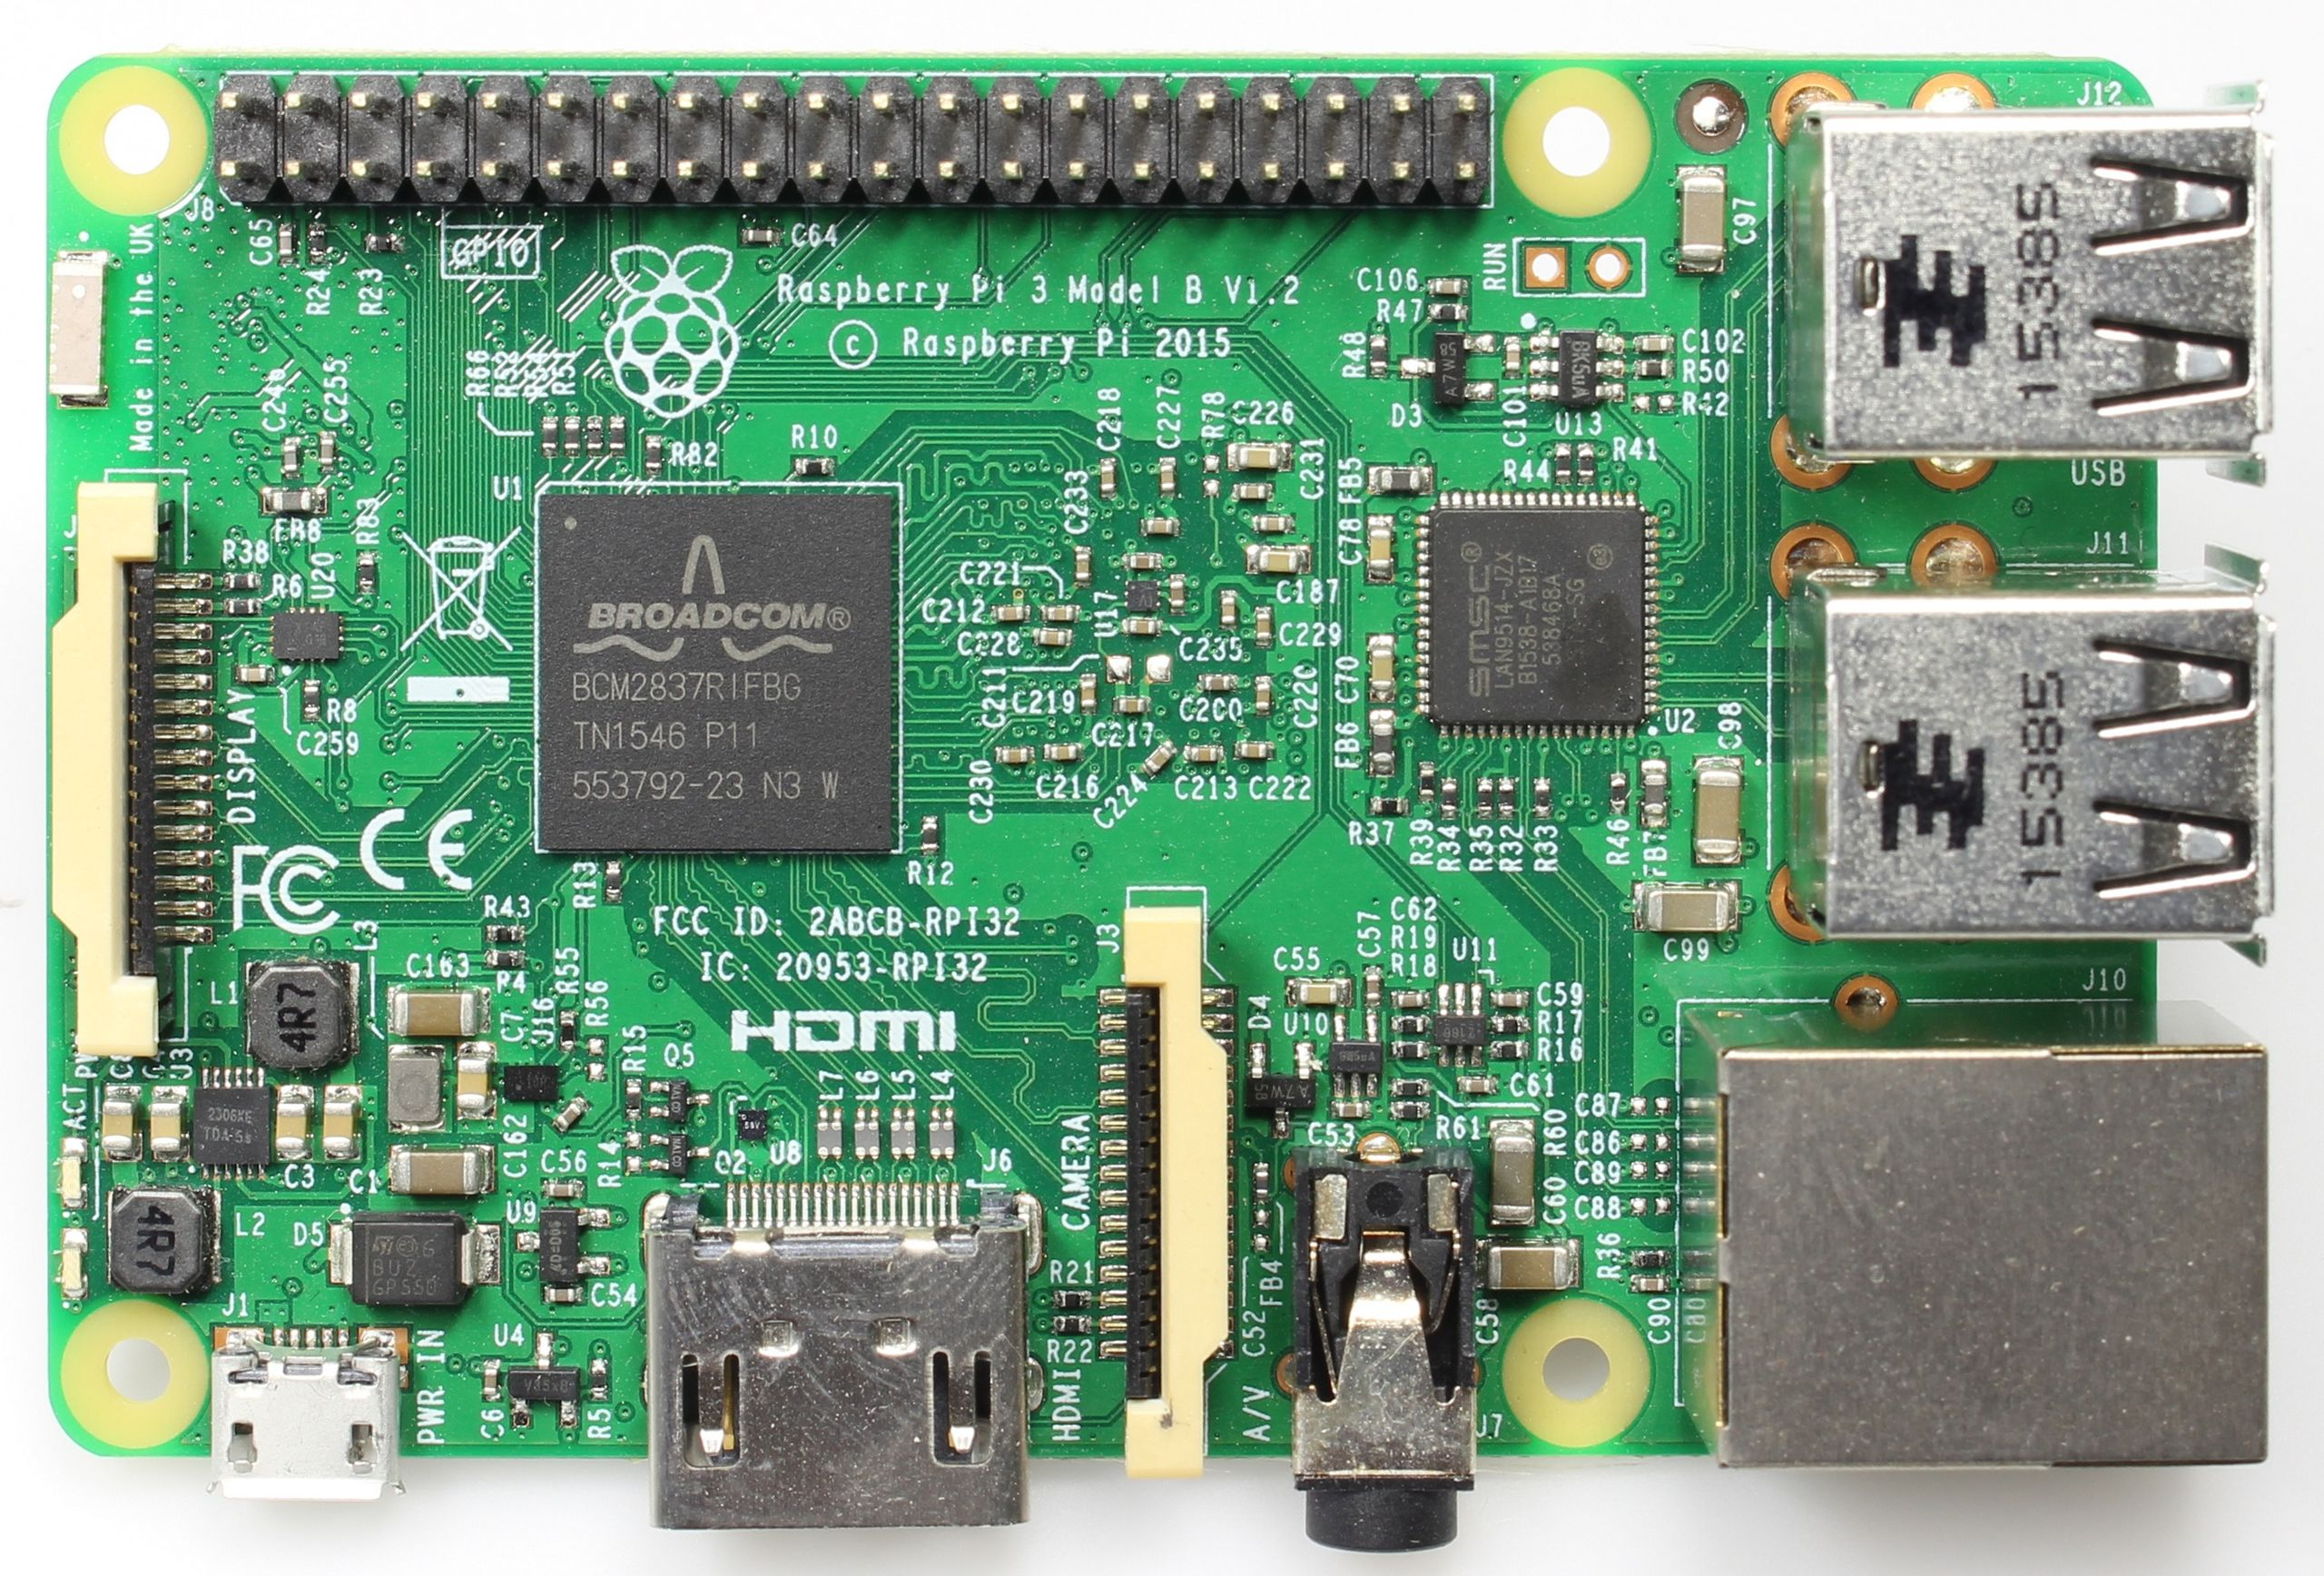
\includegraphics[scale=0.075]{img/raspi3}  %https://upload.wikimedia.org/wikipedia/commons/thumb/4/49/Rasperry_pi_3_model_b_v1.3_bot.jpg/2560px-Rasperry_pi_3_model_b_v1.3_bot.jpg
    \end{figure}

\end{frame}

\begin{frame}{Raspberry PI 3 Cluster}
	  \begin{figure}[!htb]
        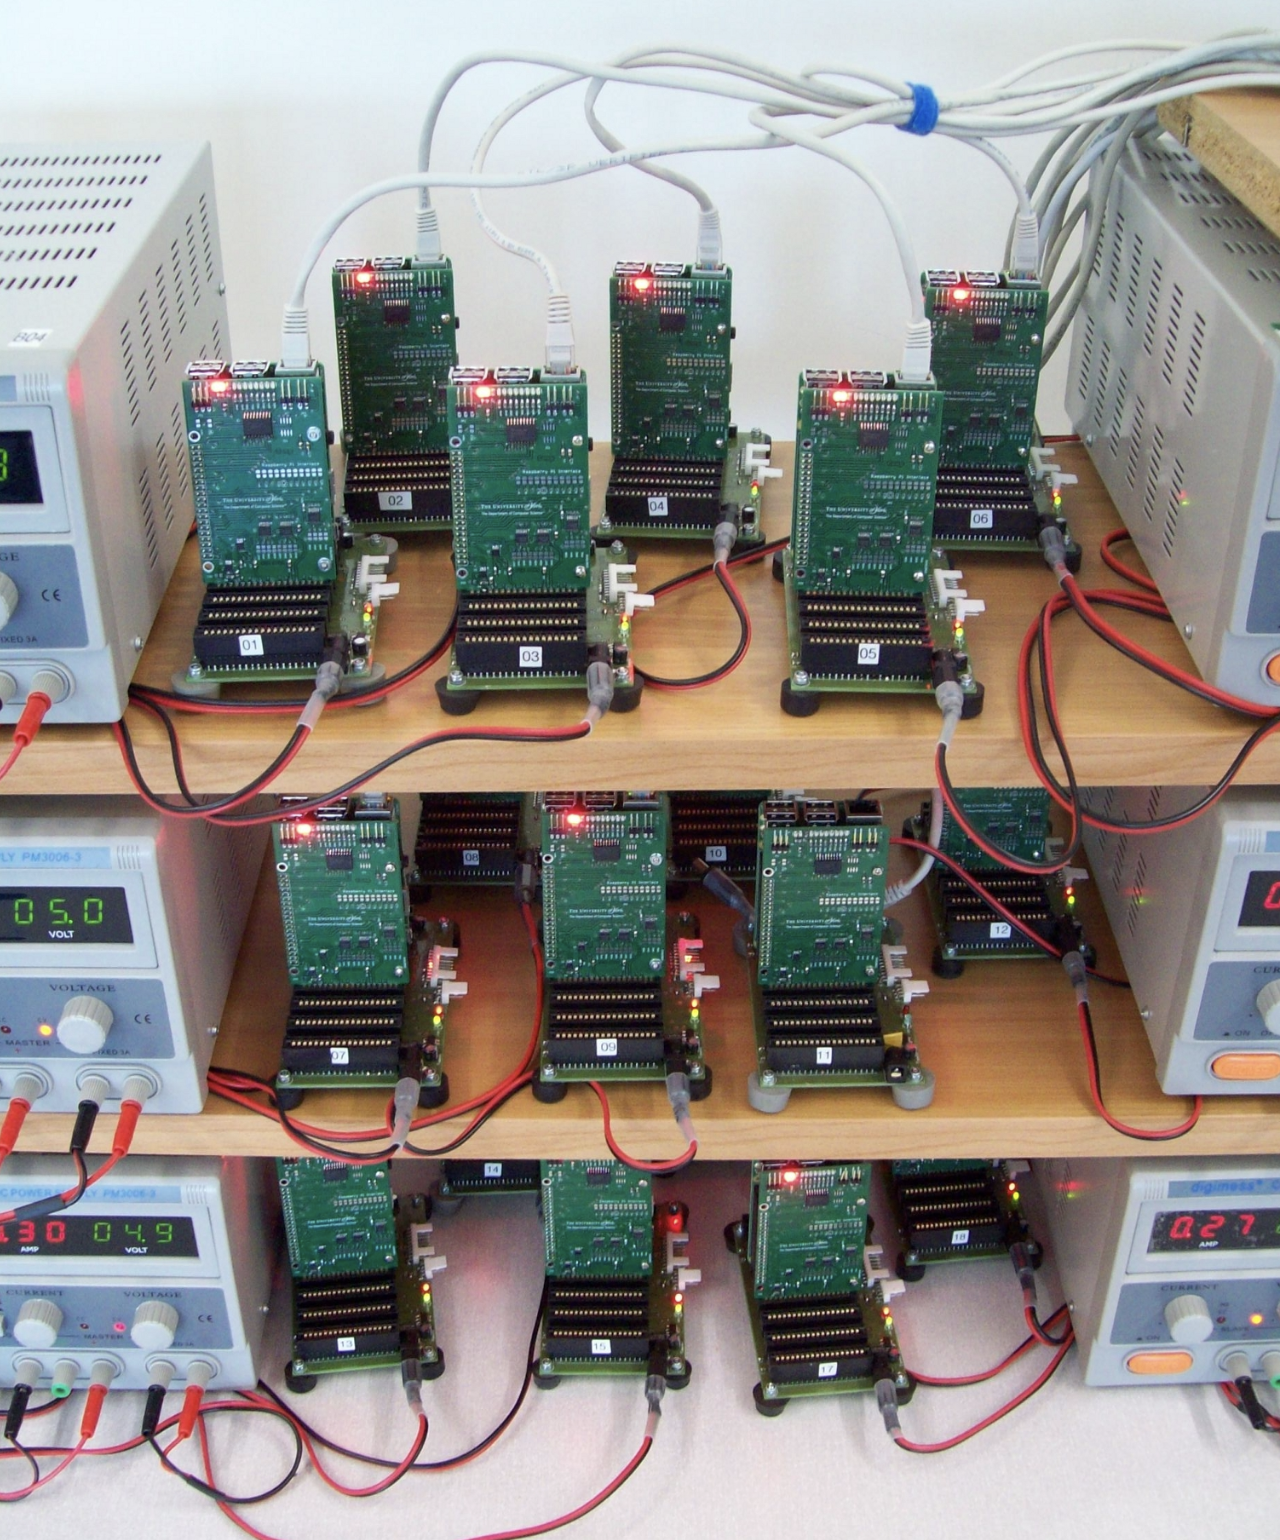
\includegraphics[scale=0.23]{img/raspi3cluster}  %https://www-users.cs.york.ac.uk/~mjf/pi_cluster/Images/cluster1.jpg
    \end{figure}

\end{frame}

\begin{frame}{Recap: Threads vs. Prozesse}

     \begin{itemize}
        \setlength{\itemindent}{1.2in}
        \item [\textbf{Definition: Prozess}]
    \end{itemize}

    \begin{itemize}
        \item Als \textbf{Prozess} definieren wir ein Programm in Ausführung, dessen Speicher und Laufzeit durch das Betriebssystem verwaltet wird
     \end{itemize}

  	   \vspace*{10mm}


         \begin{itemize}
        \setlength{\itemindent}{1.2in}
        \item [\textbf{Definition: Thread}]
    \end{itemize}

    \begin{itemize}
        \item Als \textbf{Thread} definieren wir einen nebenläufigen Teil eines Prozesses in Ausführung, dessen Speicherbereich in dem des Prozesses liegt
     \end{itemize}

    \end{frame}



\begin{frame}{Python GIL 1}
                 \begin{itemize}
        \setlength{\itemindent}{1.9in}
        \item [\textbf{Python Global Interpreter Lock }]
    \end{itemize}
    \begin{itemize}
        \item Das GIL ist ein Sperrmechanismus (Mutex mit Variable), um den Python Interpreter stets auf einen kontrollierenden Thread zu beschränken  \cite{realpython.com/python-gil}
        \item Grund: Speicherreferenzen werden in Python ermittelt und das geht mit dem GIL deterministisch $\Rightarrow$ viele Memory Leaks werden so verhindert, im Code muss man nicht ständig alles selbst mit Locks sperren
    \end{itemize}

    \end{frame}

\begin{frame}{Python GIL 2}
                 \begin{itemize}
        \setlength{\itemindent}{1.0in}
        \item [\textbf{Was heißt das? }]
    \end{itemize}
    \begin{itemize}
        \item Konsequenz:  Jeder Thread muss sich stets erst das GIL holen und kann dann laufen, weshalb CPU-lastige Aufgaben so nicht parallelisierbar sind
         \item Abhilfe:  Mit Prozessen arbeiten statt mit Threads - oder anderen Python Interpreter wählen, der ohne GIL arbeitet (kommt via Subinterpreter mit Python 3.9 in PEP-0554 \cite{python.org/dev/peps/pep-0554})
    \end{itemize}

    \end{frame}

\begin{frame}{Python Multiprocessing}
          \begin{itemize}
        \setlength{\itemindent}{1.4in}
        \item [\textbf{Multiprocessing Modul}]
    \end{itemize}
    \begin{itemize}
        \item Das Python Modul \textbf{multiprocessing} kann verwendet werden für CPU-lastige Aufgaben
        \item Aber Vorsicht: Prozess Handling ist für das Betriebssystem teurer wegen des komplexeren Kontextwechsels
        \item Hauptobjekt: Prozess $\Rightarrow$   \texttt{multiprocessing.Process(name='CalculationXY', target=my\_callback\_function)}
        \item Wichtiger Check zur Vermeidung von Endlosrekursion:   \texttt{if \_\_name\_\_ == '\_\_main\_\_'}
        \item Pool $\Rightarrow$ eine Prozessgruppe eine gemeinsame Aufgabe ausführen lassen durch Übergabe eines Callbacks
    \end{itemize}
\end{frame}

\begin{frame}{Python Multiprocessing Beispiel: Annhäherung von $\pi$} %https://gist.github.com/amitsaha/2036026
      \begin{figure}[!htb]
        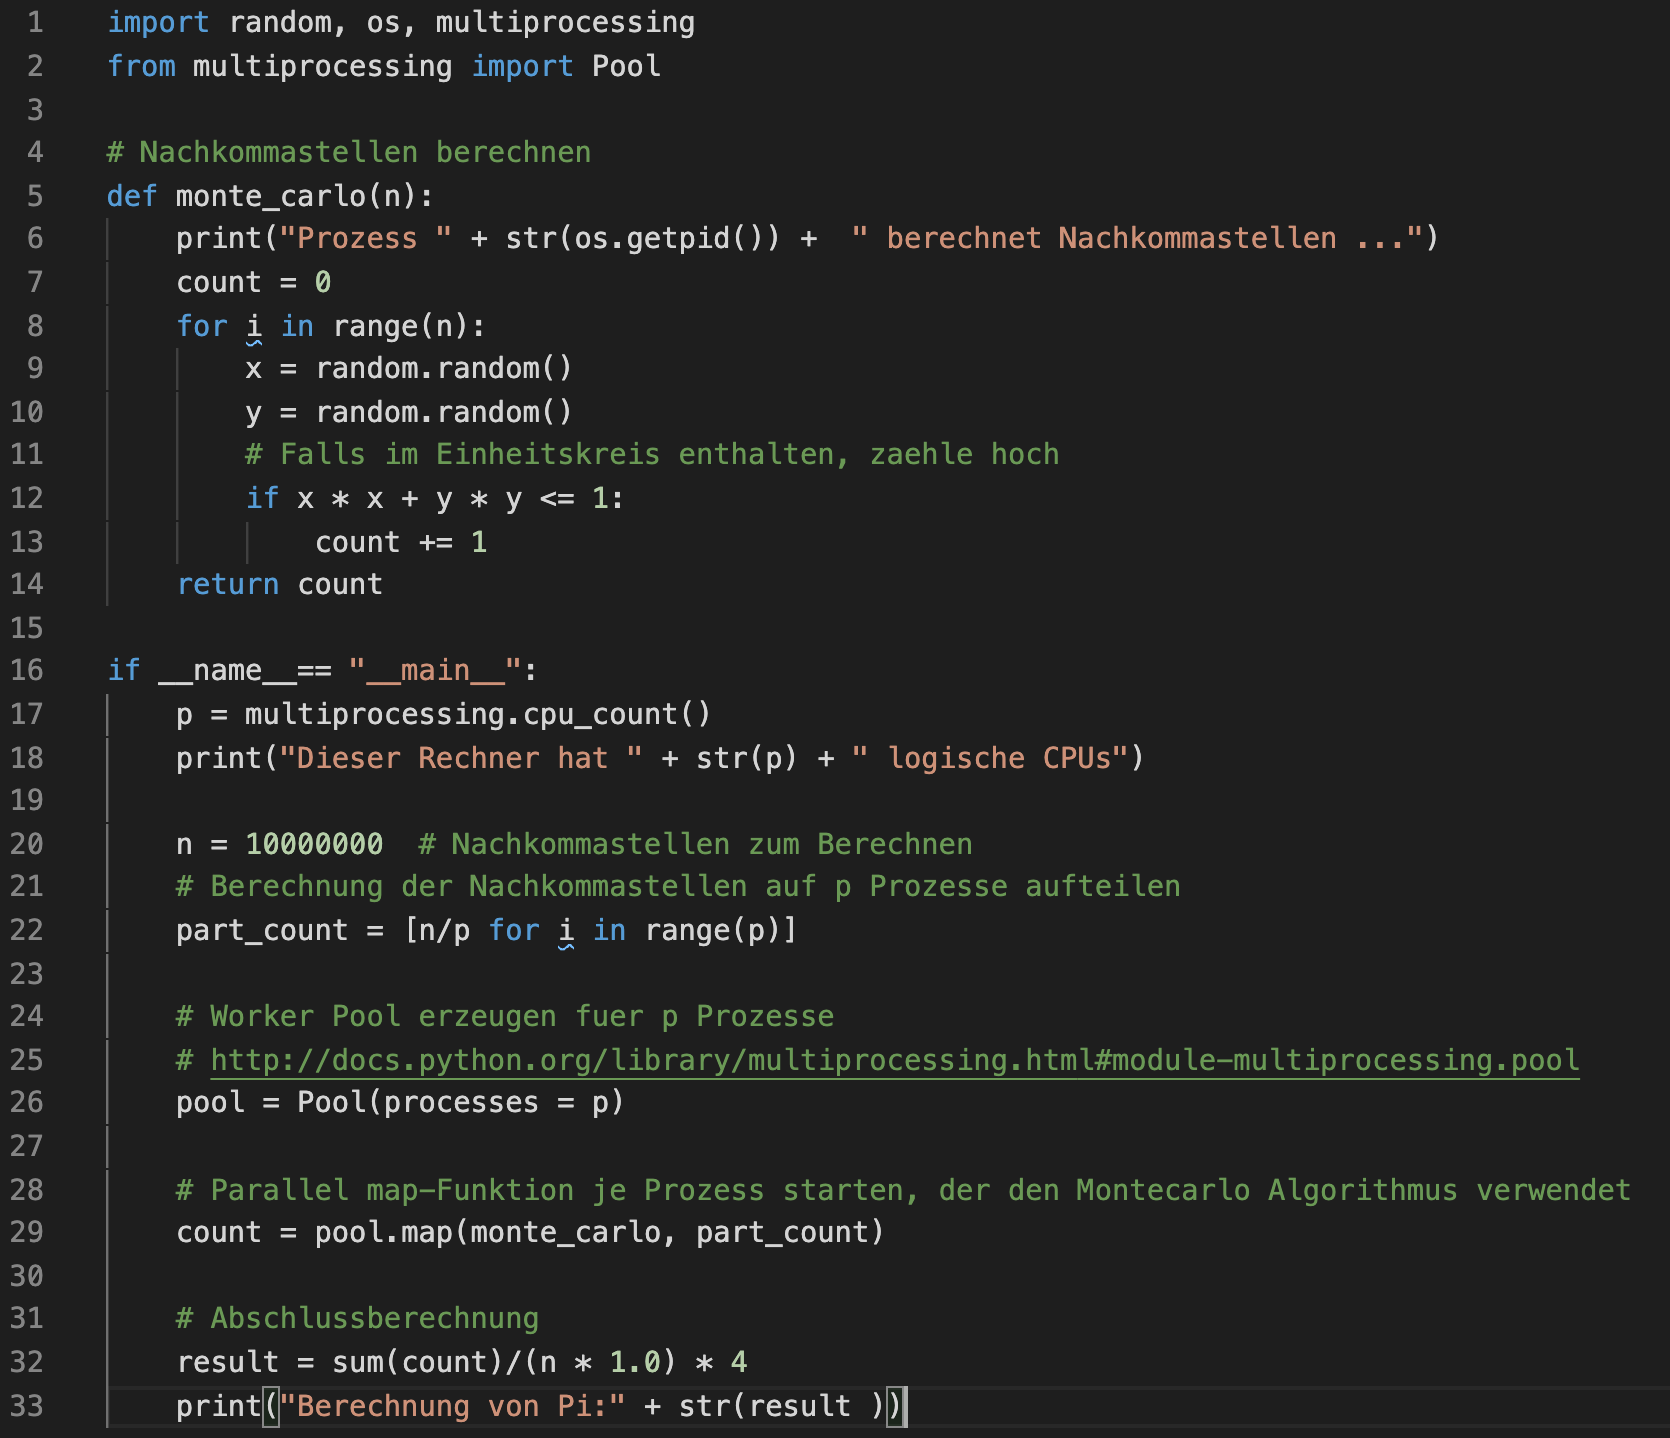
\includegraphics[scale=0.27]{img/multiprocessing_picalc}
    \end{figure}

\end{frame}

%%% Folie
\begin{frame}{Threads in Python}
         \begin{itemize}
        \setlength{\itemindent}{1.4in}
        \item [\textbf{Thread Handling Module}]
    \end{itemize}
    \begin{itemize}
        \item Das Python Modul \textbf{thread} ist das ältere Modul  mit Callbacks  $\Rightarrow$  \texttt{thread.start\_new\_thread ( cb, args[, kwargs] )}
        \item \textbf{threading} ist das modernere Modul, welches OOP verwendet und es ist in Python 3 enthalten
        \item Das Modul \textbf{threading} wird sehr ähnlich verwendet wie \textbf{multiprocessing}, mit Klassen \texttt{Thread} und \texttt{ThreadPoolExecutor}
    \end{itemize}

\end{frame}

%%% Folie
\begin{frame}{Beispiel Ping mit Threads}
  %https://www.python-kurs.eu/threads.php
    \begin{figure}[!htb]
        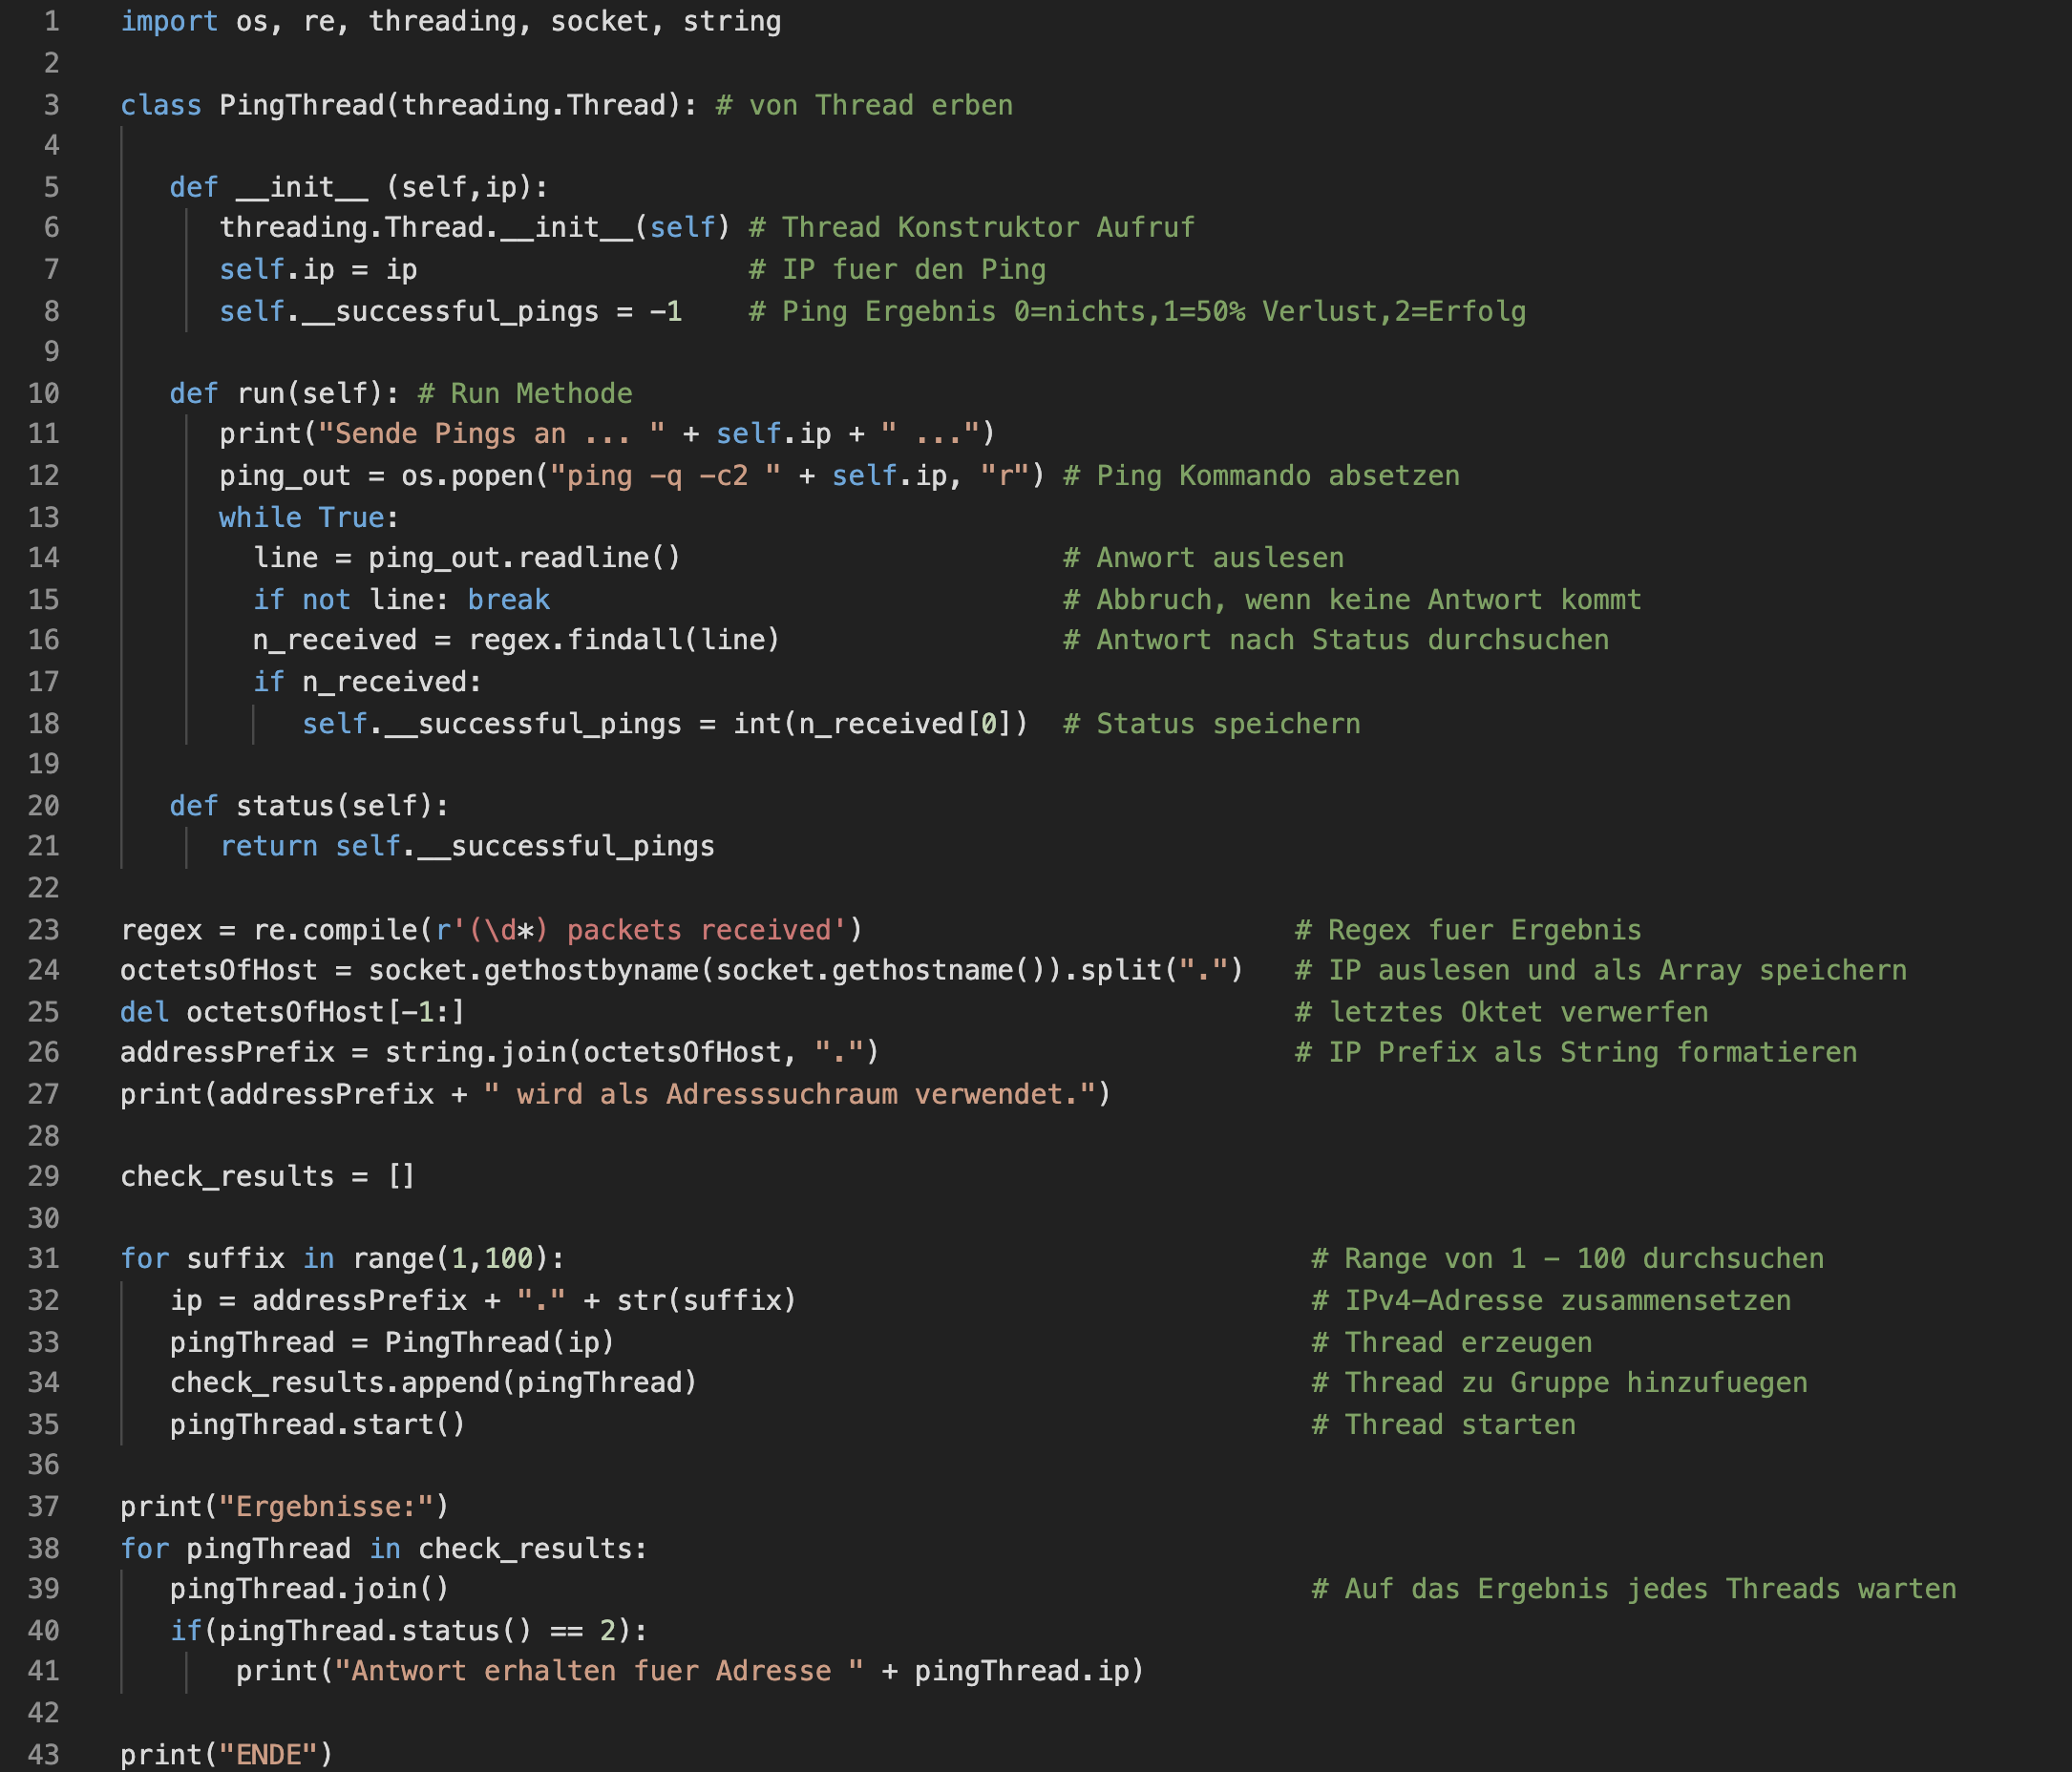
\includegraphics[scale=0.23]{img/pingthreads}
    \end{figure}

\end{frame}

%%% Folie
\begin{frame}{Thread Probleme}
         \begin{itemize}
        \setlength{\itemindent}{2.2in}
        \item [\textbf{Probleme beim Umgang mit Threads}]
    \end{itemize}
    \begin{itemize}
        \item Race Condition  $\Rightarrow$  Zugriff auf gemeinsame Daten führt  \quotes{random} zu unerwarteten Ergebnissen
        \item Lost Update $\Rightarrow$  Der letzte Schreibzugriff gewinnt
        \item Deadlock $\Rightarrow$  Jeder Thread wartet darauf, dass er die Freigabe zum laufen erhält (wurde z.B. vergessen oder ein Bug)
    \end{itemize}
\end{frame}

%%% Folie
\begin{frame}{Locking Mechanismen}
     \begin{itemize}
        \setlength{\itemindent}{2.5in}
        \item [\textbf{Locking Mechanismen aus threading Modul}]
    \end{itemize}
    \begin{itemize}
        \item \texttt{Lock}, \texttt{RLock}, \texttt{Semaphore} $\Rightarrow$  Sperren mit  \texttt{acquire(wait\_flag)}, Freigeben mit  \texttt{release()}
        \item \texttt{Event} $\Rightarrow$ ein Thread T1 wartet mit \texttt{wait()}, ein weiterer T2 setzt ein Flag via \texttt{set()}  und  T2 setzt es zurück via \texttt{clear()}
        \item \texttt{Condition} $\Rightarrow$ ein Thread T1 ruft  \texttt{acquire()} auf, wartet mit \texttt{wait()}, ein weiterer T2 ruft  \texttt{acquire()} auf,  T2 benachrichtigt via \texttt{notify()} und gibt frei mittels \texttt{release()}
        \item \texttt{with my\_lock:} statement vereinfacht die Nutzung für Locks, Condition und Semaphore $\Rightarrow$ kapselt Sperre und Freigabe
       \end{itemize}

\end{frame}


%%% Folie
\begin{frame}{Queue}
  \begin{itemize}
        \setlength{\itemindent}{1.0in}
        \item [\textbf{Das queue Modul}]
    \end{itemize}
    \begin{itemize}
        \item Enthält spezielle Klassen zur Koordination von Multithreading mit Datenaustausch zwischen den Threads
        \item \texttt{Queue}, \texttt{RLock} Abstraktion, die Intern \texttt{Condition} verwendet, um Synchonisierung zu erreichen
        \item Weitere spezialisierte Queues  \texttt{PriorityQueue}, \texttt{LifoQueue}, ...
    \end{itemize}

\end{frame}

%%% Folie
\begin{frame}{Queue Beispiel: Producer $\Rightarrow$  Consumer} %https://www.agiliq.com/blog/2013/10/producer-consumer-problem-in-python/
     \begin{figure}[!htb]
        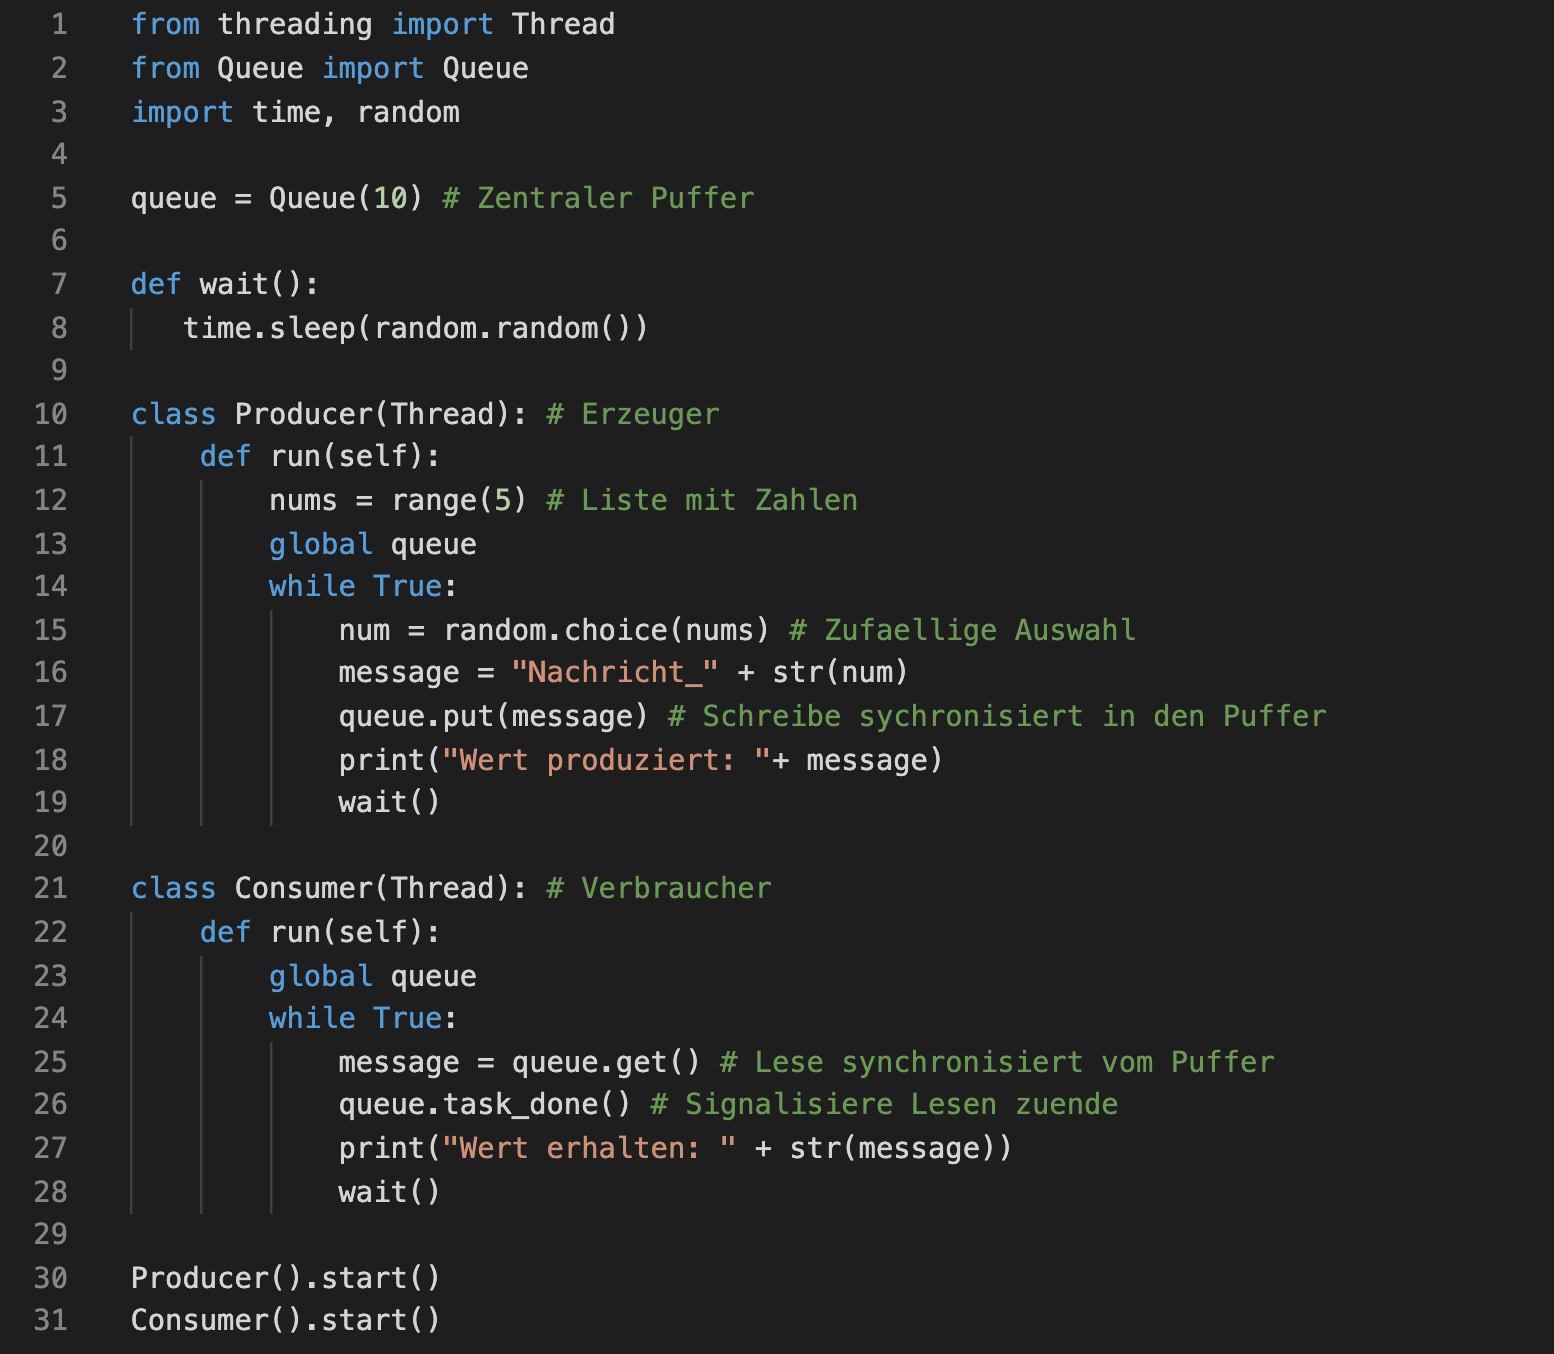
\includegraphics[scale=0.31]{img/producerconsumer}
    \end{figure}
\end{frame}

%%% Folie
\begin{frame}{Nebenläufigkeit für I/O Tasks}
     \begin{itemize}
        \setlength{\itemindent}{1.2in}
        \item [\textbf{Das asyncio Modul}]
    \end{itemize}
    \begin{itemize}
        \item Nebenläufigkeit innerhalb eines Threads $\Rightarrow$ Kein Kontextwechsel via Scheduler, sondern \textbf{Eventloop} (ähnlich zu JavaScript)
        \item \texttt{async} Keyword macht Funktionen zu Coroutines, die unterbrechbar sind
        \item Das Ergebnis bekommt man mit \texttt{await}
        \item Mithilfe der Loop lassen sich \textbf{Futures} über  \texttt{loop.create\_task} erzeugen (ähnlich zu Promises in JavaScript oder Futures in Java)
        \item Weitere Libraries bauen darauf auf, z.B. \texttt{aiohttp} für HTTP Requests
      \end{itemize}

\end{frame}


%%% Folie
\begin{frame}{Beispiel Coroutines: Abfrage Wetterdaten für Städte} %https://dev.to/welldone2094/async-programming-in-python-with-asyncio-12dl
         \begin{figure}[!htb]
           \hspace*{-0.5cm}
        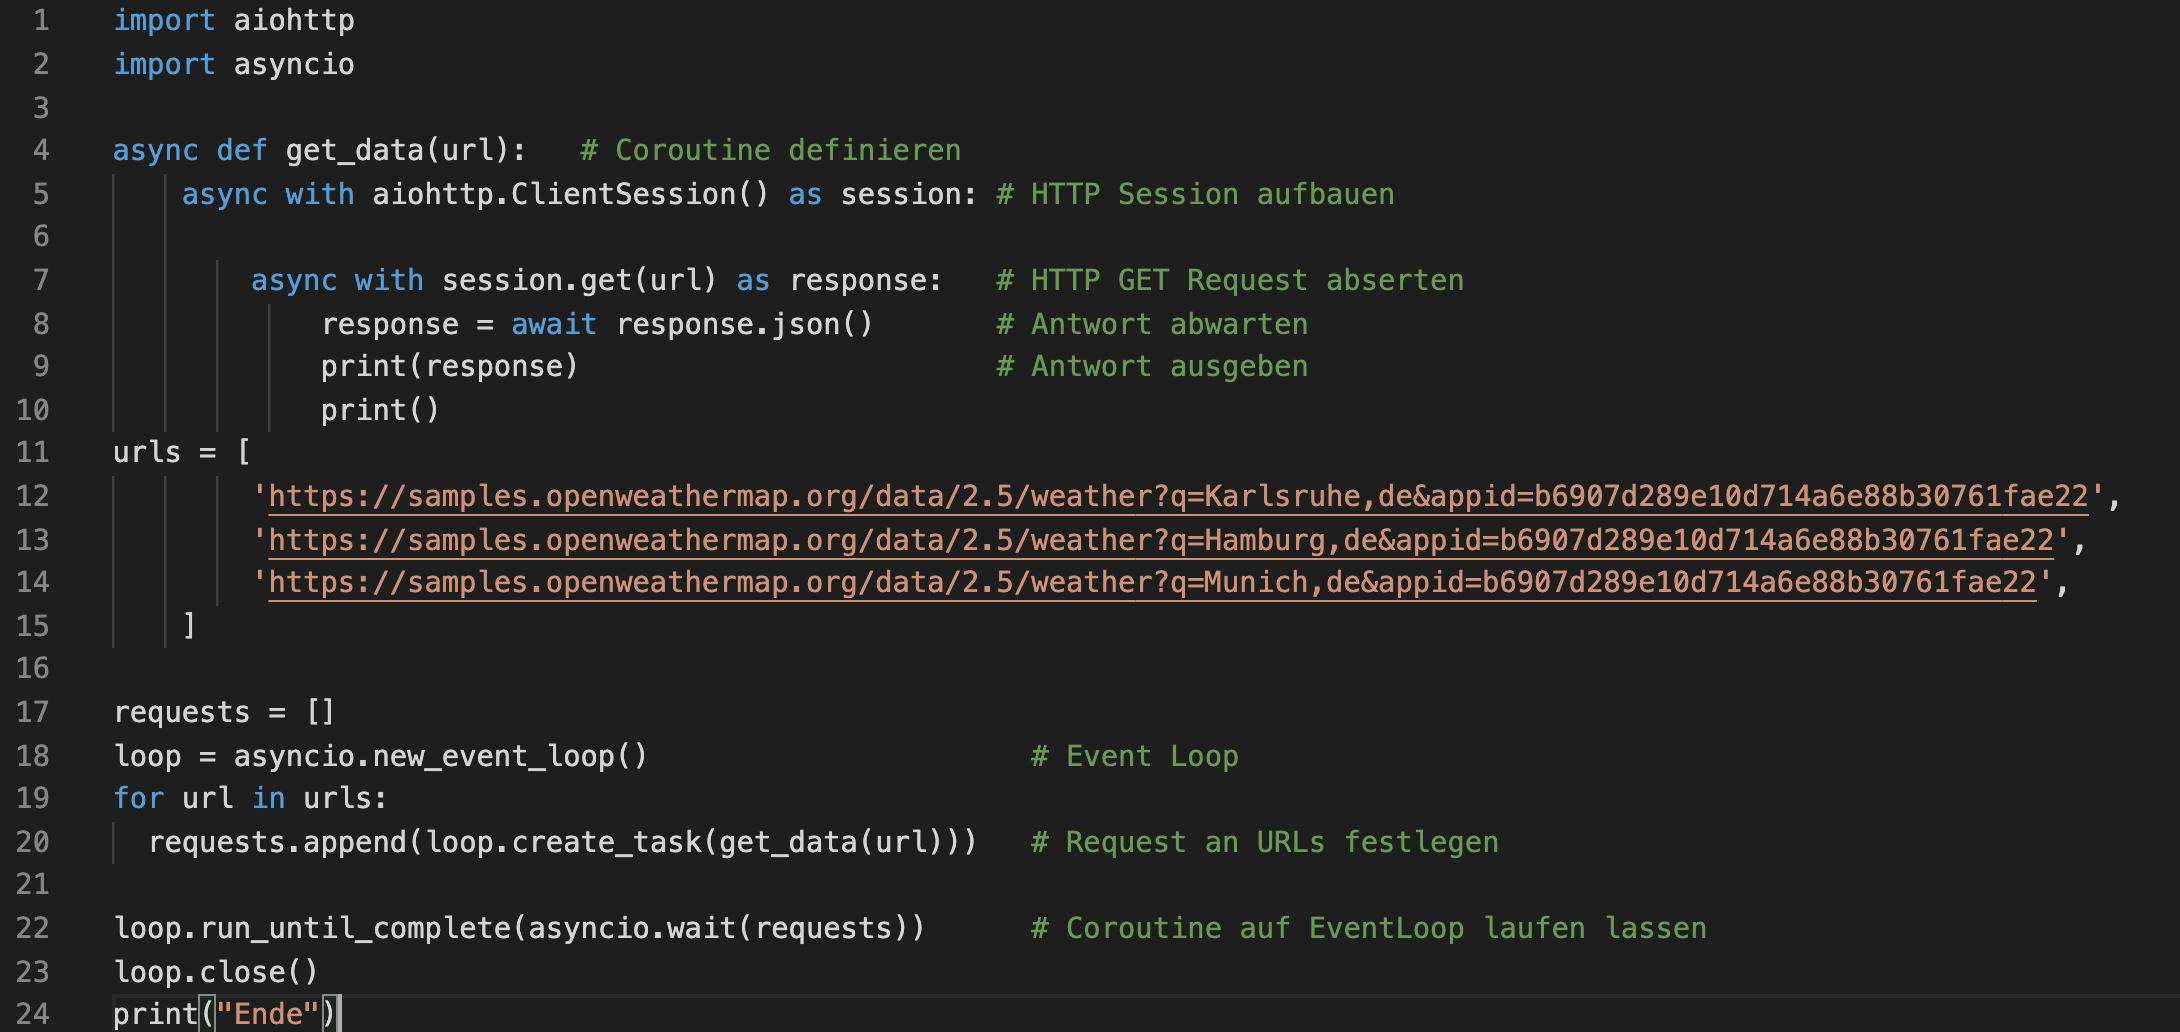
\includegraphics[scale=0.31]{img/coroutine_download}
    \end{figure}
\end{frame}



%%% Folie
\begin{frame}{Zusammenfassung Nebenläufigkeit}

  \begin{itemize}
        \setlength{\itemindent}{2.2in}
        \item [\textbf{Welches Konstrukt wann verwenden?}]
    \end{itemize}
    \begin{itemize}
        \item I/O-lastig? (Netzwerk, Sensorik, Dateien) $\Rightarrow$ \texttt{asyncio}, eventuell erweitert um \texttt{uvloop}
        \item CPU-lastig? (teure Berechnungen) $\Rightarrow$ \texttt{multiprocessing}
        \item Alle weiteren Fälle $\Rightarrow$ \texttt{threading}
    \end{itemize}

\end{frame}
